\begin{figure}[ht!]
\centering
% --------- P ---------
\begin{minipage}[b]{0.33\textwidth}
\raggedright
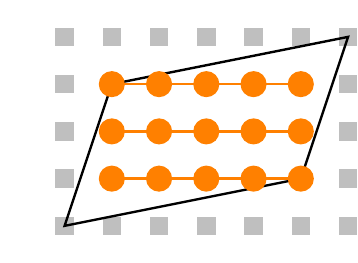
\begin{tikzpicture}[scale=0.6]\vspace{0.5cm}
\hspace{1em}
\foreach \x in {0,...,6} {
    \foreach \y in {0,...,4} {
        \node at (\x,\y) [fill=lightgray, minimum width=2pt] {};   
    }
}
\draw[line width=0.3mm, black] (0,0) -- (1,3) -- (6,4) -- (5,1) -- cycle;

\draw[line width=0.3mm, orange] (1,1) -- (5,1);
\draw[line width=0.3mm, orange] (1,2) -- (5,2);
\draw[line width=0.3mm, orange] (1,3) -- (5,3);


\foreach \x in {1,...,5} {
    \node at (\x,1) [circle, fill=orange, minimum width=3pt] {};
    \node at (\x,2) [circle, fill=orange, minimum width=3pt] {};
    \node at (\x,3) [circle, fill=orange, minimum width=3pt] {};
}
\end{tikzpicture}
\end{minipage}%
% --------- 2P ---------
\begin{minipage}[b]{0.33\textwidth}
\centering
\begin{tikzpicture}[scale=0.3]\vspace{0.5cm}
\foreach \x in {0,...,12} {
    \foreach \y in {0,...,8} {
        \node at (\x,\y) [circle, draw=white, fill=lightgray, minimum width=2.5pt] {};   
    }
}
\draw[line width=0.3mm, black] (0,0) -- (2,6) -- (12,8) -- (10,2) -- cycle;


\draw[line width=0.3mm, darklav] (1,2) -- (10,2);
\draw[line width=0.3mm, darklav] (1,3) -- (10,3);
\draw[line width=0.3mm, darklav] (2,5) -- (11,5);
\draw[line width=0.3mm, darklav] (2,6) -- (11,6);

\foreach \x in {1,...,10} {
    \node at (\x,2) [circle, fill=darklav, minimum width=3pt] {};
    \node at (\x,3) [circle, fill=darklav, minimum width=3pt] {};
}
\foreach \x in {2,...,11} {
    \node at (\x,5) [circle, fill=darklav, minimum width=3pt] {};
    \node at (\x,6) [circle, fill=darklav, minimum width=3pt] {};
}

\end{tikzpicture}
\end{minipage}%
% --------- 3P ---------
\begin{minipage}[b]{0.33\textwidth}
\raggedleft
\begin{tikzpicture}[scale=0.2]\vspace{0.5cm}
\foreach \x in {0,...,18} {
    \foreach \y in {0,...,12} {
        \node at (\x,\y) [circle, draw=white, fill=lightgray, minimum width=2.2pt] {};   
    }
}
\draw[line width=0.3mm, black] (0,0) -- (3,9) -- (18,12) -- (15,3) -- cycle;


\draw[line width=0.3mm, lightgreen] (1,3) -- (15,3);
\draw[line width=0.3mm, lightgreen] (2,6) -- (16,6);
\draw[line width=0.3mm, lightgreen] (3,9) -- (17,9);

\foreach \x in {1,...,15} {
    \node at (\x,3) [circle, fill=lightgreen, minimum width=3pt] {};
}
\foreach \x in {2,...,16} {
    \node at (\x,6) [circle, fill=lightgreen, minimum width=3pt] {};
}
\foreach \x in {3,...,17} {
    \node at (\x,9) [circle, fill=lightgreen, minimum width=3pt] {};
}
\end{tikzpicture}
\hspace{1em}
\end{minipage}
\caption{Lattice diameter segments in dilates of $P$ to visualize the values $n_i,\rem_i,r_i$ and $\blocks_i$.}
\label{fig:dilations-123}
\end{figure}